\subsubsection{The problem of Pipeline Hazards}\label{subsubsection: The problem of Pipeline Hazards}

\begin{definitionbox}[: Hazard]
    A \indexdefinition{hazard (conflict)} is created whenever there a \textbf{dependence} between two instructions, and instructions are close enough that the overlap caused by pipelining would change the order of access to the operands involved in the dependence.
\end{definitionbox}

\begin{flushleft}
    \textcolor{Red2}{\faIcon{exclamation-triangle} \textbf{Problem Consequences}}
\end{flushleft}
The Hazards:
\begin{itemize}
    \item \textbf{Force} the next \textbf{instruction} in the pipeline \textbf{to be executed later} than its intended clock cycle.

    \item \textbf{Reduced the performance} from the ideal speedup achieved by pipelining (direct previous consequence).
\end{itemize}
There are \textbf{three classes} of Hazards:
\begin{itemize}
    \item \indexdefinition{Structural Hazards}. Attempt to use the \textbf{same resource from different instructions simultaneously}.
    
    \example{Example}: single memory for instruction and data.
    

    \item \indexdefinition{Data Hazards}. Attempt to \textbf{use a result before it is ready}.
    
    \example{Example}: instruction depending on a result of a previous instruction still in the pipeline.

    There are also \textbf{two specific forms} of data hazard, called \indexdefinition{Load-Use Data Hazard} and \indexdefinition{Load-Store Data Hazard}. Both occur when the \textbf{data loaded by a load instruction is not yet available when it is needed by another instruction}. In the case of Load-Use, the \dquotes{another instruction} is an operator such as \texttt{add}; in the case of Load-Store, the \dquotes{another instruction} is the store (\texttt{sw}) instruction.

    The following \example{example} shows the conflict (Load-Use Data Hazard) between two instructions. In particular, the value \texttt{lw} writes to \texttt{s2} is not available until \texttt{lw} has completed the \texttt{MEM} phase, but \texttt{and} needs this value when it enters the \texttt{EX} phase, i.e. when \texttt{lw} enters the \texttt{MEM} phase.
    \lstinputlisting[language=misc]{code/the-problem-of-pipeline-hazards/load-use-data-hazard.s}

    \item \indexdefinition{Control Hazards}. Attempt to \textbf{make a decision on the next instruction to execute before the condition is evaluated} (more detailed analysis on page \pageref{flushleft: how to detect Control Hazards}).
    
    \example{Example}: conditional branch execution.
\end{itemize}

\begin{flushleft}
    Structural Hazards? No problem for MIPS Architecture!
\end{flushleft}
\textbf{There aren't any structural hazards in MIPS architecture} because the Instruction Memory (IM) is separated from the Data Memory (DM). Also, the Register File (RF) is used in the same clock cycle (read access by an instruction and write access by another instruction).

\newpage

\begin{flushleft}
    \textcolor{Green3}{\faIcon{question-circle} \textbf{How to detect \underline{Data Hazards}? Dependency Analysis}}
\end{flushleft}
To \textbf{detect Data Hazards}, it is suggested to analyze the dependencies. If the instructions executed in the pipeline depend on each other, data hazards can arise \textbf{when instructions are too close}. For \example{example}:
\lstinputlisting[language=misc]{code/the-problem-of-pipeline-hazards/data-hazards-1.s}
Data Hazards can occur in a variety of situations, but a \textbf{true dependency situation} is created by a \textbf{RAW (Read After Write) Hazard}.

\begin{definitionbox}[: Read After Write Hazard]
    A \indexdefinition{RAW (Read After Write) Hazard} occurs when an instruction $n+1$ tries to read a source operand before the previous instruction $n$ has written its value in the Register File (RF).
\end{definitionbox}

\noindent
For \example{example}:
\lstinputlisting[language=misc]{code/the-problem-of-pipeline-hazards/RAW-hazard-1.s}

\newpage

\begin{flushleft}
    \textcolor{Green3}{\faIcon{question-circle} \textbf{How to detect \underline{Control Hazards}? Check conditional branches}}
    \label{flushleft: how to detect Control Hazards}
\end{flushleft}
First of all, some \example{examples} of conditional branches for MIPS processor are: \texttt{beq} (branch on equal) and \texttt{bne} (branch on not equal):
\lstinputlisting[language=misc]{code/mips-architecture/beq-bne.s}
The \textbf{address to which you want to branch} is called the \indexdefinition{Branch Target Address}. If the branch condition:
\begin{itemize}
    \item Is satisfied $\Rightarrow$ the \textbf{branch is taken} and the Branch Target Address is stored in the Program Counter (PC).

    \item Is \underline{not} satisfied $\Rightarrow$ the \textbf{branch is not taken} (untaken) and the instruction stream is executed sequentially with the next instruction address (PC $+ 4$).
\end{itemize}
In detail, the stages are the following:
\begin{enumerate}
    \item \texttt{[IF]} Instruction fetch and PC increment.
    \item \texttt{[ID]} Instruction Decode and Registers Read (e.g. \texttt{x} and \texttt{y})
    \item \texttt{[EX]} Compare registers (e.g. \texttt{x} and \texttt{y}) in the ALU to derive the Branch Outcome: taken or not taken. Also, computation of the Branch Target Address, so $\texttt{PC} + 4 + \texttt{offset}$
    \item \texttt{[ME]} The Branch Outcome is used to decide the next PC:
    \begin{itemize}
        \item Is satisfied $\Rightarrow$ \texttt{PC} take $\texttt{PC} + 4 + \texttt{offset}$
        \item Is \underline{not} satisfied $\Rightarrow$ \texttt{PC} take $\texttt{PC} + 4$
    \end{itemize}
\end{enumerate}
Let us now move on to a more interesting analysis. To understand when the Control Hazards occur, think about the Branch Outcome and the Branch Target Address. Both are ready at the end of the EX (execution) phase (so between pass number 3 and 4). Finally, branches are resolved when the Program Counter is updated at the end of the Memory Access stage (after pass number 4). 

\highspace
To feed the condition branch into the pipeline, we need to \textbf{create a way where the condition branch is decided before the EX stage of the next instruction}. It's obvious, because if the Branch Outcome is positive, we need to skip the next instruction and do the conditional jump instead.

\highspace
This is a more detailed explanation of a control hazard. Control Hazards arise from the pipelining of conditional branches and other \texttt{jump} \textbf{instructions that change the PC}. They also \textbf{reduce the performance from the ideal speedup gained by pipelining}, because it is necessary to hold the pipeline until the branch is resolved.

\newpage

\begin{center}
    \large
    \textcolor{Red3}{\textbf{MIPS Optimized Pipeline}}
\end{center}
Consider the following situation:
\begin{figure}[!htp]
    \centering
    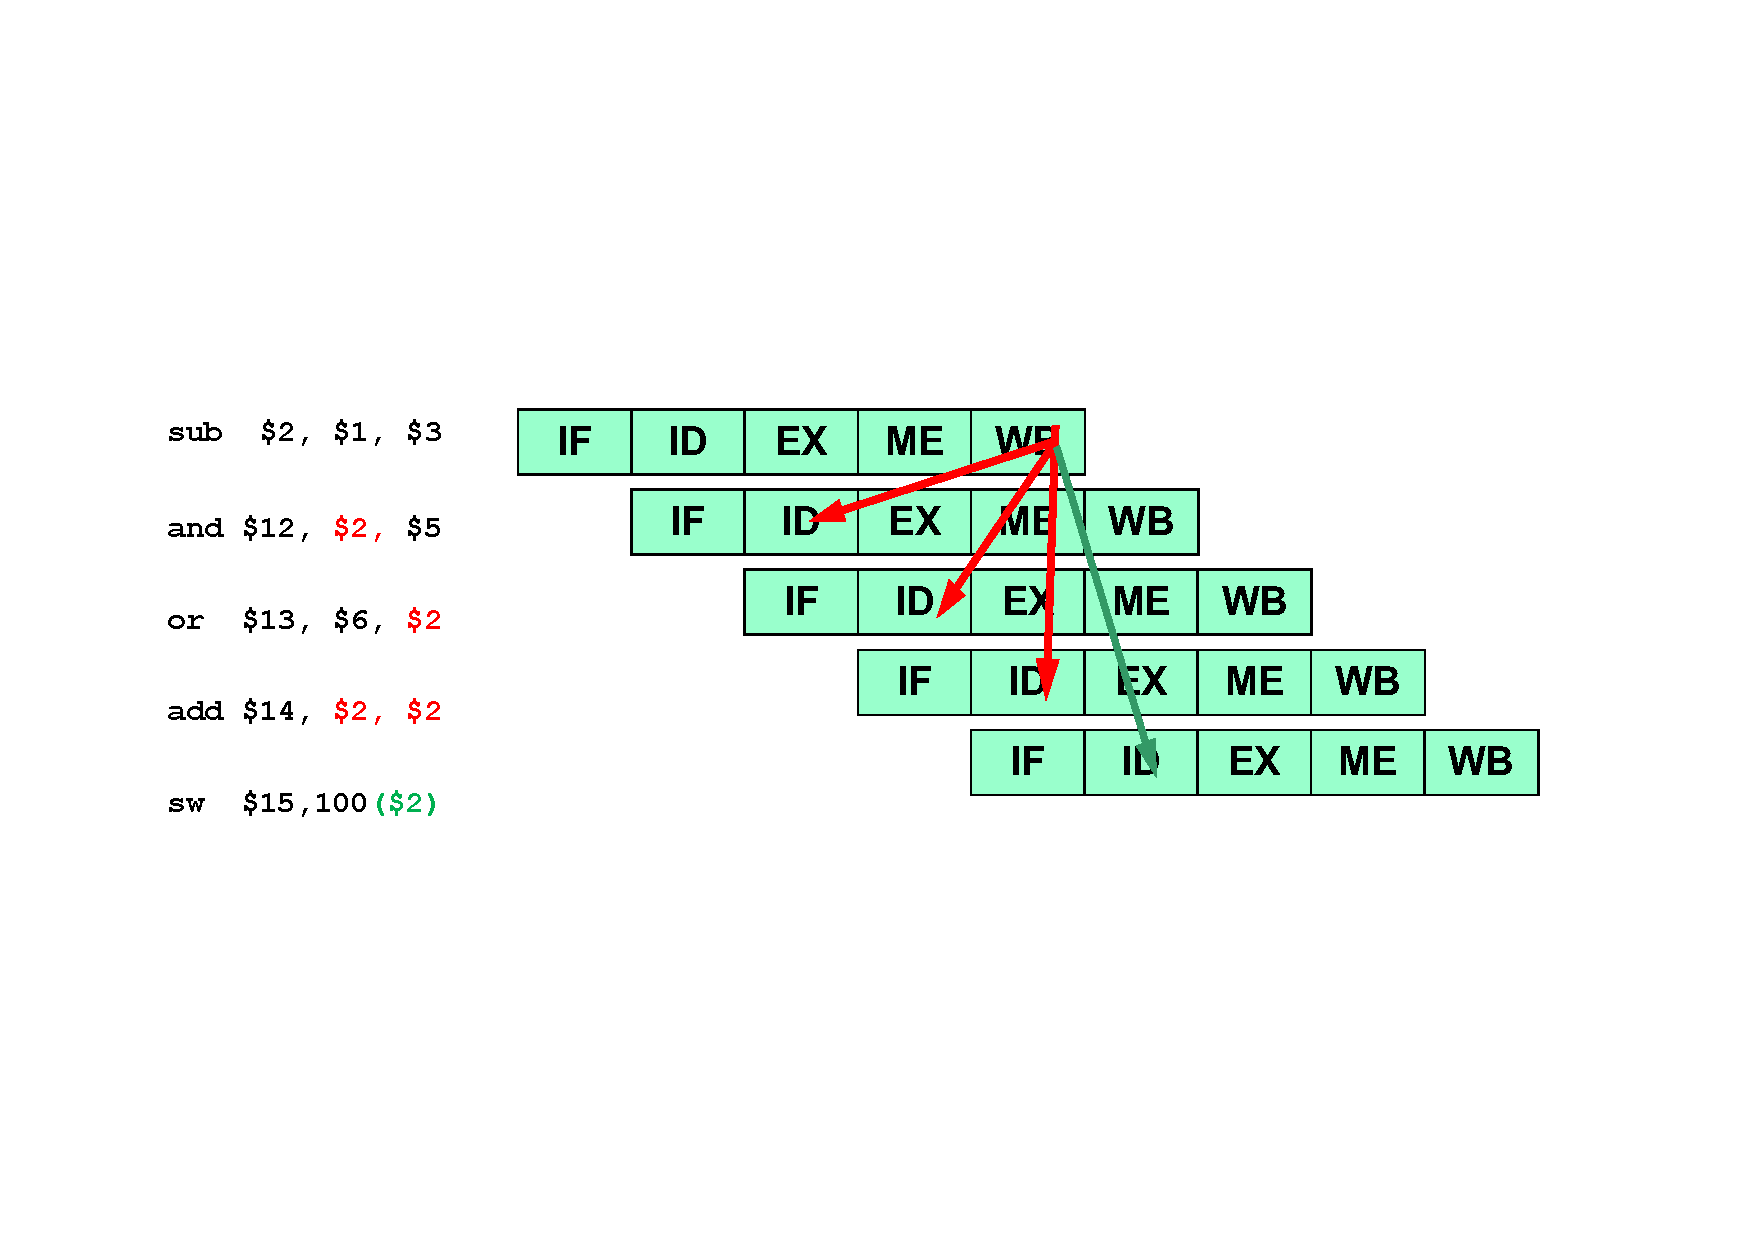
\includegraphics[width=\textwidth]{img/RAW-hazards-1.pdf}
    \caption{Why MIPS Optimized Pipeline was born.\cite{pipelining-slides}}
\end{figure}

\noindent
The Register File is used in 2 stages: read access during ID (\texttt{and} operation) and write access during Write Back (WB) (\texttt{sub} operation). \emph{What happens if read and write refer to the same register in the same clock cycle?} Or we insert a stall, or we use an \textbf{optimized pipeline} (smart choice).

\begin{definitionbox}[: Optimized Pipeline]
    By selecting \indexdefinition{Optimized Pipeline}, we assume the Register File (RF) read occurs in the second half of clock cycle and the Register File write in the first half of clock cycle.
\end{definitionbox}

\noindent
This way \textbf{we don't need the stall}. The following Figure~\ref{fig: Optimized Pipeline} shows an optimized pipeline.

\newpage

\begin{figure}[!htp]
    \centering
    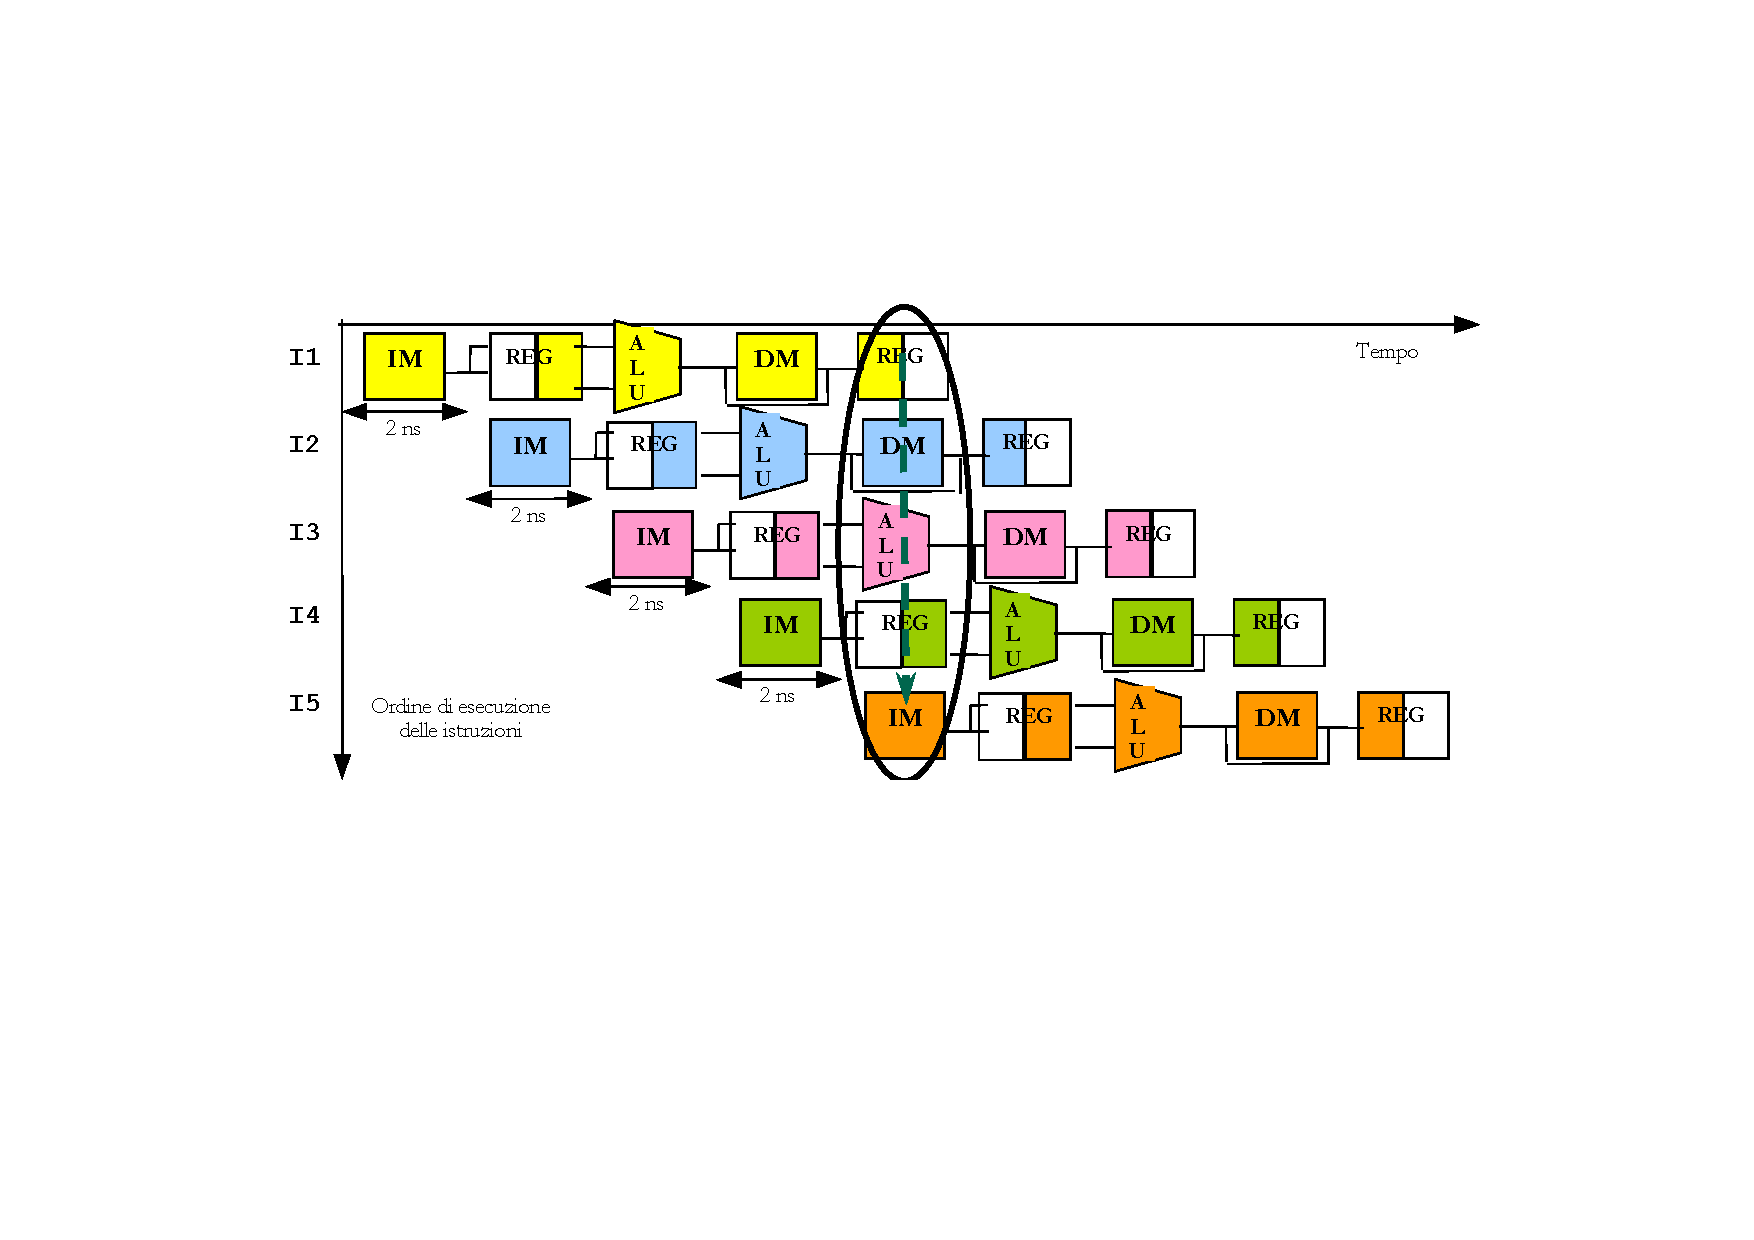
\includegraphics[width=\textwidth]{img/optimized-pipeline-1.pdf}
    \caption{Optimized Pipeline (IM is Instruction Memory, REG is Register File, and DM is Data Memory).\cite{pipelining-slides}}
    \label{fig: Optimized Pipeline}
\end{figure}

\noindent
And the problem mentioned at the beginning of this paragraph is partially solved, as we can see in the following figure.
\begin{figure}[!htp]
    \centering
    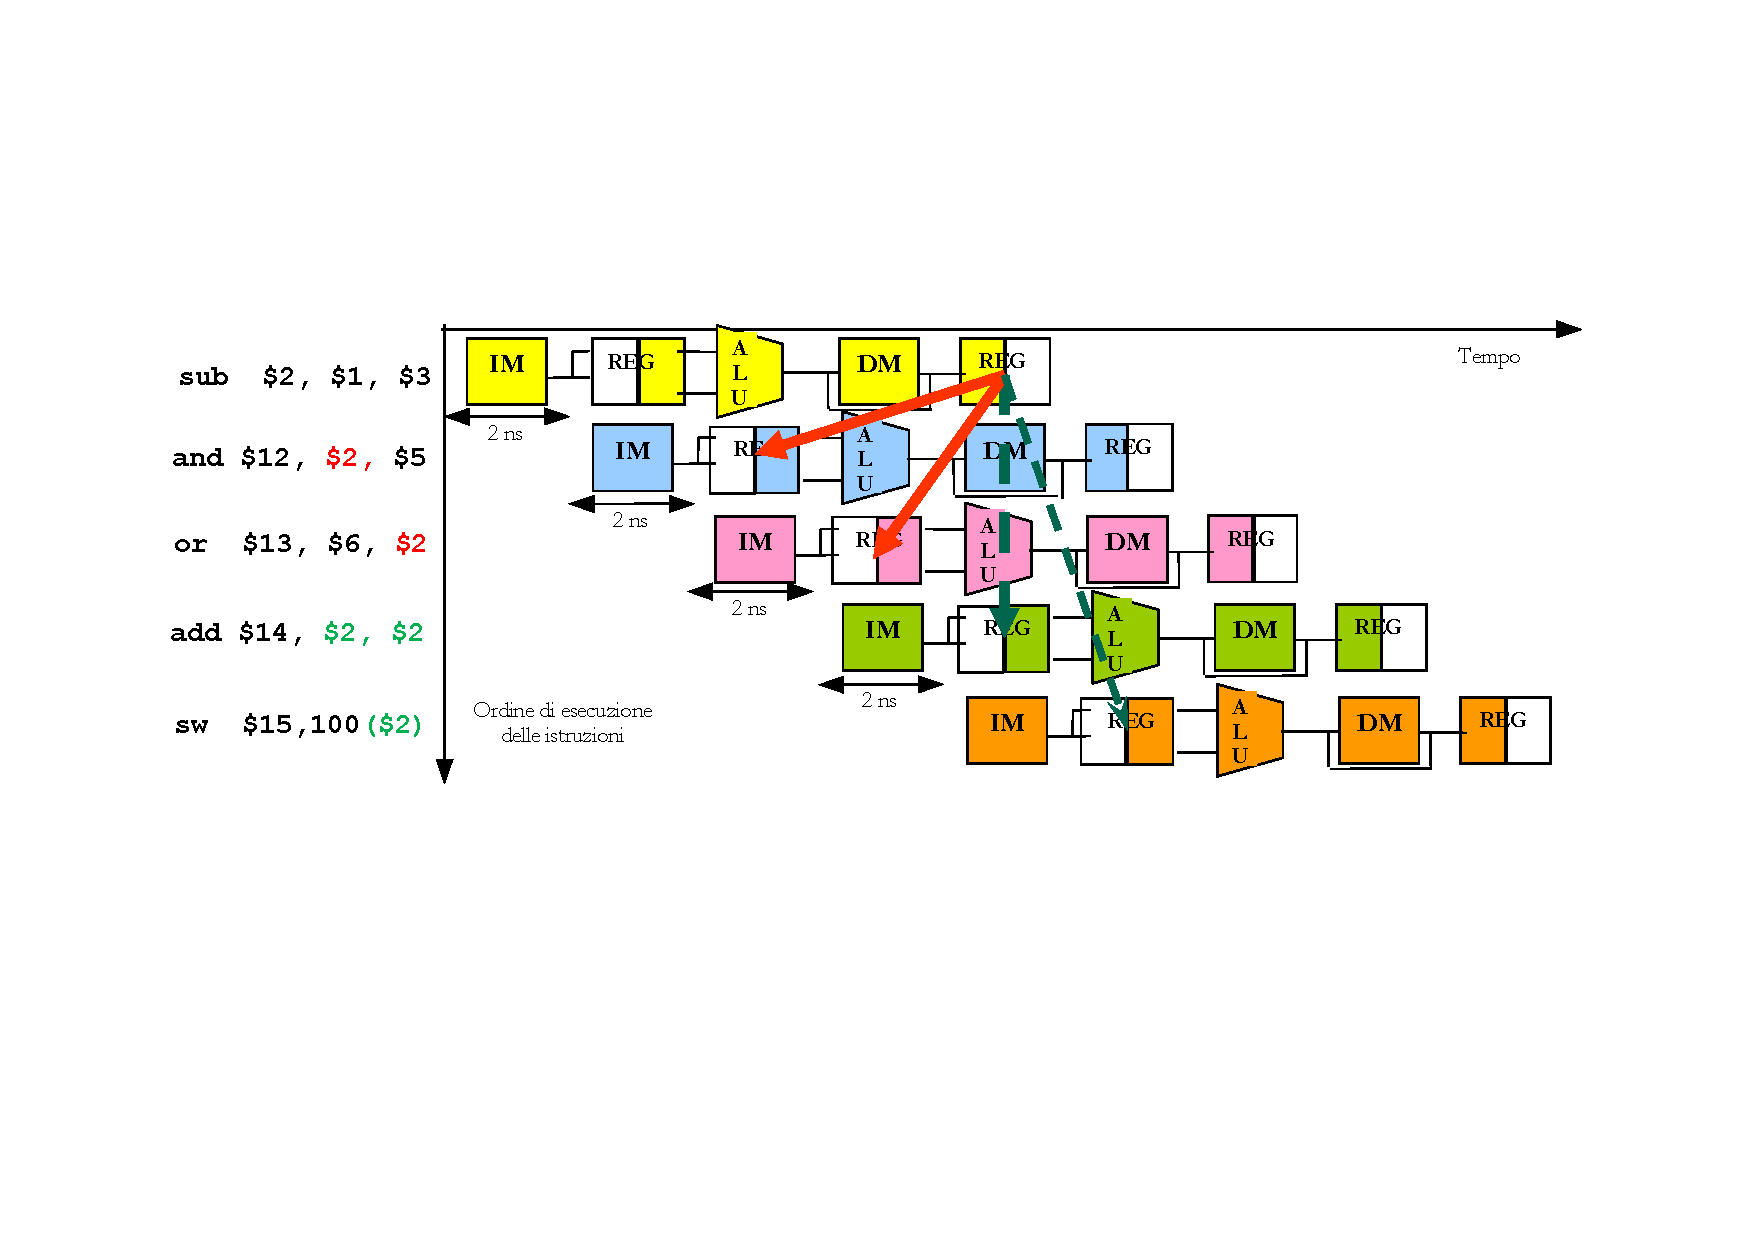
\includegraphics[width=\textwidth]{img/optimized-pipeline-2.pdf}
    \caption{Optimized Pipeline to solve the example stall.\cite{pipelining-slides}}
\end{figure}